\chapter{푸리에 쌍대성, 운동량, 자유입자 운동}

\section{기초에서 예제로}

얽힘은 양자역학의 핵심에 놓여 있지만, 이제 기초를 충분히 살펴보았으므로 이를 활용하기 시작할 수 있다. 지금까지 이 강의에서는 스핀, 회전 가능한 장치, 유한한 결과 목록, 확률을 추론하기 위한 반복 측정처럼 의도적으로 작은 계에 의존해 왔다. 이런 실험은 양자역학이 발견된 역사적 경로보다 논리적으로 단순하지만, 작동 원리를 이루는 최소한의 요소를 담고 있다.

\begin{classroomqa}
\audiencequestion{양자역학에서 뉴턴 역학의 몇 가지 경험적 출발점에 해당하는 것은 무엇인가?}
\lecturerresponse{최소 모형은 회전 가능한 스핀 측정 장치다. 스핀을 준비하고, 축을 선택한 다음, 측정 버튼을 누르고, \(+1\) 또는 \(-1\)를 기록한다. 결과의 빈도를 알 수 있을 때까지 실험을 반복하면 된다. 벡터 공간, 관측량, 진폭, 보른 규칙은 이러한 통계를 정리해 준다. 역사적으로 이론은 훨씬 풍부한 원자 현상에서 비롯되었지만, 논리적으로는 이 두 결과를 갖는 실험만으로도 이론의 구조를 드러내기에 충분하다.}
\end{classroomqa}

\begin{classroomqa}
\audiencequestion{스핀이나 운동량처럼 물리량이 달라질 때마다 같은 통계적 절차를 수행해야 하나요?}
\lecturerresponse{그렇다. 관측량은 특정한 실험 장치의 종류와 가능한 결과에 대응한다. 상태와 관측량을 지정하면 형식론이 확률분포를 예측하지만, 관측량의 물리적 의미는 그것을 어떻게 측정하는지에 근거한다.}
\end{classroomqa}

얽힘을 마무리하기 전에 앞선 논의에서 나온 한 가지 질문에 완전히 답해 두자. 두 전자의 단일항 및 삼중항 부문을 생각하고, 복사장을 또 하나의 양자 부분계로 포함하자. 복사장에는 진공 상태 \(\ket{0_\gamma}\)와 광자 하나가 있는 상태 \(\ket{1_\gamma}\)가 있다. 입자 수 자체도 중첩될 수 있다. 중첩을 입자 수가 고정된 상태들 사이로만 제한하는 규칙은 없다.

수업에서 논의한 이상화된 전이의 경우, 처음에 얽히지 않은 전자 상태는 단일항 성분과 삼중항 성분의 중첩으로 쓸 수 있다.
\begin{equation}
\ket{\uparrow\downarrow}
=
\frac{1}{\sqrt{2}}
\left(\ket{S}+\ket{T_0}\right).
\end{equation}
처음에 광자가 없으면 상태는 다음과 같다.
\begin{equation}
\ket{\Psi(0)}
=
\frac{1}{\sqrt{2}}
\left(\ket{S}+\ket{T_0}\right)
\otimes\ket{0_\gamma}.
\label{eq:l9-initial-radiative-state}
\end{equation}
단일항 성분은 방출 없이 단일항으로 남지만, 들뜬 삼중항 성분은 단일항으로 이완하면서 광자를 방출할 수 있다.
\begin{align}
\ket{S}\ket{0_\gamma}
&\longrightarrow
\ket{S}\ket{0_\gamma}, \\
\ket{T_0}\ket{0_\gamma}
&\longrightarrow
\ket{S}\ket{1_\gamma}.
\end{align}
그러면 선형성에 따라 다음을 얻는다.
\begin{equation}
\ket{\Psi_{\mathrm{final}}}
=
\ket{S}\otimes
\frac{\ket{0_\gamma}+\ket{1_\gamma}}{\sqrt{2}}.
\label{eq:l9-final-radiative-state}
\end{equation}

\begin{figure}[htbp]
\centering
\includegraphics[width=0.88\textwidth]{lecture_09_figure_01.png}
\caption{복사 이완 전에 전자 상태를 단일항 성분과 삼중항 성분으로 분해하고 광자 진공 상태와 텐서곱한다.}
\lectureframe{00:05:10}
\end{figure}

마지막 식은 전자쌍과 복사장 사이의 곱 상태다. \(\ket{S}\)가 얽혀 있으므로 두 전자는 서로 얽혀 있고, 복사장은 광자가 0개인 상태와 1개인 상태의 중첩으로 남는다. 이 예는 상호작용이 얽힘을 재분배한다는 점에서 미묘하다. 처음의 전자 곱 상태는 얽힌 전자쌍으로 진화하지만, 이상화한 최종 전자-복사장 상태는 인수분해된다.

\begin{classroomqa}
\audiencequestion{들어오는 광자라면 어떤 것이든 전이를 되돌려 전자들의 얽힘을 풀 수 있나요?}
\lecturerresponse{아니다. 시간 역전 과정에는 적절한 광자 상태와 모드, 위상, 에너지, 상호작용 이력이 필요하다. 방출된 광자를 되비춘다는 말은 닫힌 계 전체의 역방향 시간 진화를 구현한다는 뜻을 간략히 표현한 것이지, 임의의 광자가 얽힘을 풀어 준다는 뜻은 아니다.}
\end{classroomqa}

\begin{classroomqa}
\audiencequestion{외부 자기장을 도입하지 않았는데 삼중항 상태가 방출하는 이유는 무엇인가요?}
\lecturerresponse{전자들은 서로, 그리고 양자화된 전자기장과 상호작용한다. 스핀에 의존하는 상호작용 때문에 한 스핀 배열의 에너지가 더 낮아지고, 남는 에너지는 복사로 빠져나갈 수 있다. 외부 측정 장치는 필요하지 않다. 이는 전자와 장을 합친 계의 통상적인 유니터리 동역학이다.}
\end{classroomqa}

남은 문제를 정리했으니 이제 스핀은 잊고 가장 단순한 운동 문제, 즉 일차원 직선 위의 입자 하나를 살펴보자.

\section{평면파와 푸리에 쌍}

물리학으로 돌아가기 전에 수학을 잠시 살펴보자. 다음 식에서 시작하자.
\begin{equation}
e^{ipx}=\cos(px)+i\sin(px).
\end{equation}
이 단계에서 \(p\)는 진동률을 정하는 실수일 뿐이다. 이 식에는 시간 의존성이 없으므로 아직 움직이는 파동을 나타내지는 않는다. \(x\)의 함수로 보면 익숙한 사인파 형태를 띠므로 평면파라고 부른다.

충분히 매끄러운 함수는 이런 모드들로 분해할 수 있다. 아래 적분이 잘 정의될 만큼 적절히 거동하는 함수만 고려하자. 공간 무한대에서 발산해서는 안 되며, 뒤에서 다룰 물리적 파동 함수는 제곱적분 가능하다. 대칭 정규화 관례를 쓰면 푸리에 쌍은 다음과 같다.
\begin{align}
\psi(x)
&=
\int_{-\infty}^{\infty}
\frac{dp}{\sqrt{2\pi}}\,
\widetilde{\psi}(p)e^{ipx},
\label{eq:l9-fourier-forward}\\
\widetilde{\psi}(p)
&=
\int_{-\infty}^{\infty}
\frac{dx}{\sqrt{2\pi}}\,
\psi(x)e^{-ipx}.
\label{eq:l9-fourier-inverse}
\end{align}
계수 \(\widetilde{\psi}(p)\)는 푸리에 변수 \(p\)에 해당하는 모드의 복소 진폭이다. \(1/\sqrt{2\pi}\)의 인자는 관례에 따른다. 양방향 변환에 하나씩 두면 두 식이 서로 대칭적으로 보인다. 지수의 상대적인 마이너스 부호는 필수적이다.

\begin{figure}[htbp]
\centering
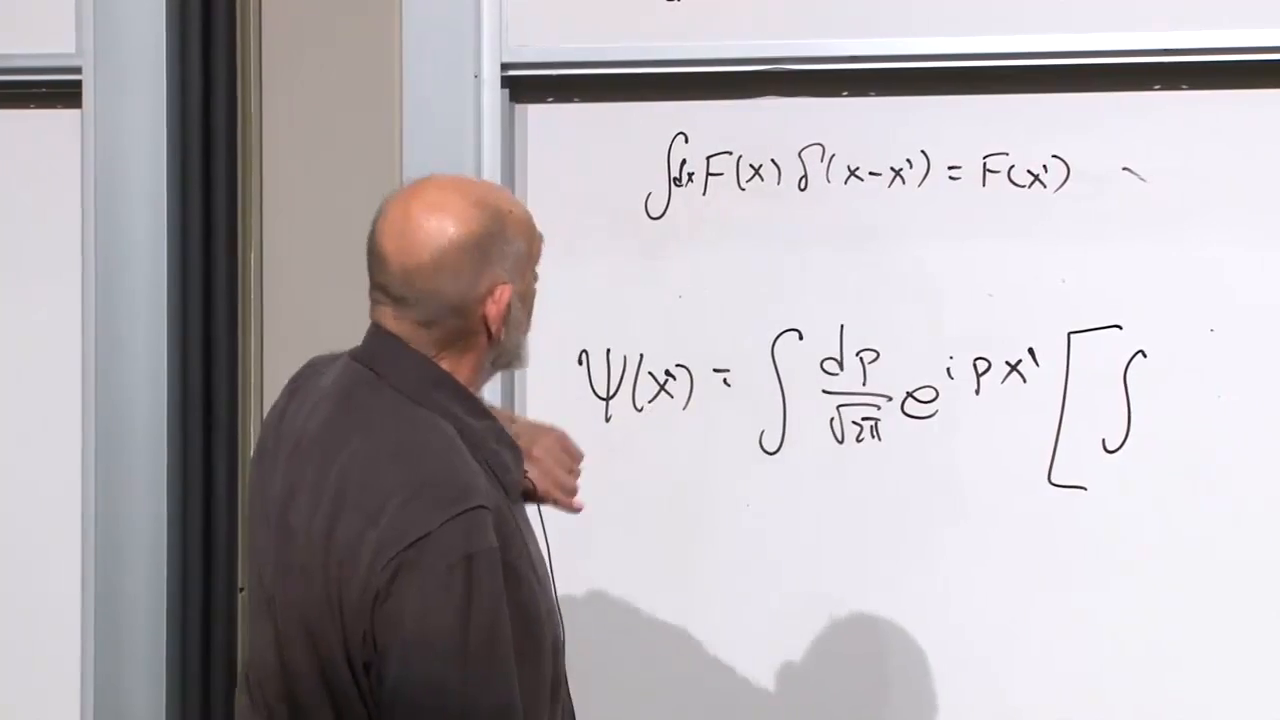
\includegraphics[width=0.88\textwidth]{lecture_09_figure_02.png}
\caption{대칭 푸리에 쌍: 함수를 평면파들로 분해하고 역변환으로 각 모드의 진폭을 구한다.}
\lectureframe{00:14:35}
\end{figure}

\begin{classroomqa}
\audiencequestion{\(\psi(x)\)와 \(\widetilde{\psi}(p)\)는 복소수인가요?}
\lecturerresponse{일반적으로 그렇다. 특수한 함수는 실수일 수 있으며, 이 경우 푸리에 계수는 켤레 관계를 추가로 만족한다. 그러나 양자 진폭은 자연스럽게 복소수이고, 여기서는 실수로 제한하지 않는다.}
\end{classroomqa}

\begin{classroomqa}
\audiencequestion{왜 대칭 인자 \(1/\sqrt{2\pi}\)를 사용하나요? \(2\pi\)를 한쪽 변환에 모두 넣을 수도 있지 않나요?}
\lecturerresponse{어느 관례를 써도 일관성이 있다. 대칭 관례를 쓰면 정방향 변환과 역변환은 지수의 부호만 달라진다. 관련된 모든 정규화를 일관되게 바꾸기만 하면 물리적 예측은 관례에 좌우되지 않는다.}
\end{classroomqa}

\(x\)와 \(p\) 사이의 상호적 관계가 이미 드러난다. 한 함수를 다른 변수에 대해 적분하여 나타낼 수 있다. 지금은 이것이 푸리에 해석이다. 곧 이 두 변수는 위치와 운동량이 된다.

\section{연산으로서의 디랙 델타}

직관적으로 델타 함수는 폭이 한없이 좁아지고 높이가 발산하며 면적은 단위 면적인 뾰족한 봉우리로 그릴 수 있다. 이런 그림은 유용하지만, 연산을 통해 내리는 정의가 더 신뢰할 만하다. 적절한 시험 함수 \(f\)에 대해
\begin{equation}
\int_{-\infty}^{\infty}
dx\,\delta(x-x')f(x)
=f(x').
\label{eq:l9-delta-sampling}
\end{equation}
익숙한 세 가지 규칙은 같은 생각을 나타낸다.
\begin{align}
f(x)\delta(x-x')
&=
f(x')\delta(x-x'),
\label{eq:l9-delta-multiplication}\\
\int_{-\infty}^{\infty}dx\,\delta(x-x')
&=1,
\label{eq:l9-delta-area}\\
\int_{-\infty}^{\infty}dx\,\delta(x-x')f(x)
&=f(x').
\end{align}
첫 번째 규칙이 성립하는 것은 델타 함수가 \(x=x'\)인 곳에서만 지지집합을 갖기 때문이다. 두 번째 규칙에서는 뾰족한 봉우리의 위치가 바뀌어도 면적은 변하지 않는다. 이 두 규칙을 결합하면 세 번째 규칙을 얻는다.

\begin{figure}[htbp]
\centering
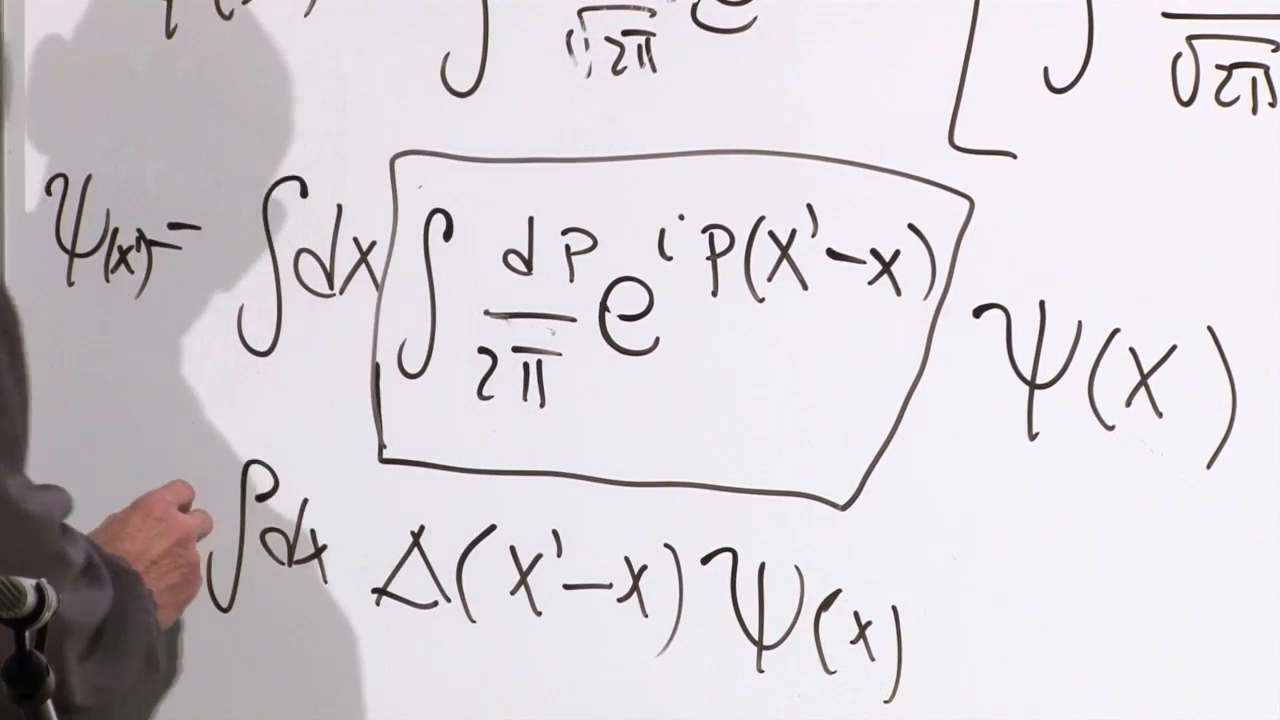
\includegraphics[width=0.88\textwidth]{lecture_09_figure_03.png}
\caption{적절한 모든 함수에 대한 작용으로 정의되는 디랙 델타의 표본 추출 성질.}
\lectureframe{00:19:45}
\end{figure}

\begin{classroomqa}
\audiencequestion{왜 \(f(x')\)을 \(x\) 적분 기호 밖으로 꺼낼 수 있나요?}
\lecturerresponse{적분 변수는 \(x\)입니다. 적분하는 동안 \(x'\)는 고정되어 있으므로 \(f(x')\)은 \(x\)에 대한 상수입니다. 나머지 델타 함수 적분의 면적은 단위 면적입니다.}
\end{classroomqa}

델타 함수는 보통의 점별 함수가 아니다. 특히 이를 제곱하면 원래 델타 함수보다 더 특이한 대상이 된다. 안전한 의미는 분포의 의미다. 식~\eqref{eq:l9-delta-sampling}은 적분 안에서 델타 함수가 어떻게 작용하는지를 규정한다.

\subsection{델타 함수의 푸리에 표현}

식~\eqref{eq:l9-fourier-inverse}을 식~\eqref{eq:l9-fourier-forward}에 대입하고, 좌변의 변수 이름을 \(x'\)로 바꾸자.
\begin{align}
\psi(x')
&=
\int\frac{dp}{\sqrt{2\pi}}\,
e^{ipx'}
\left[
\int\frac{dx}{\sqrt{2\pi}}\,
\psi(x)e^{-ipx}
\right] \notag\\
&=
\int dx
\left[
\int\frac{dp}{2\pi}
e^{ip(x'-x)}
\right]\psi(x).
\label{eq:l9-fourier-composition}
\end{align}
대괄호 안의 식은 적절한 모든 \(\psi\)에 대해 \(\psi(x')\)를 재현해야 한다. 델타 함수의 정의에 따른 작용과 비교하면 다음을 얻는다.
\begin{equation}
\boxed{
\int_{-\infty}^{\infty}
\frac{dp}{2\pi}\,
e^{ip(x'-x)}
=\delta(x'-x)
}.
\label{eq:l9-delta-fourier-x}
\end{equation}

\begin{figure}[htbp]
\centering
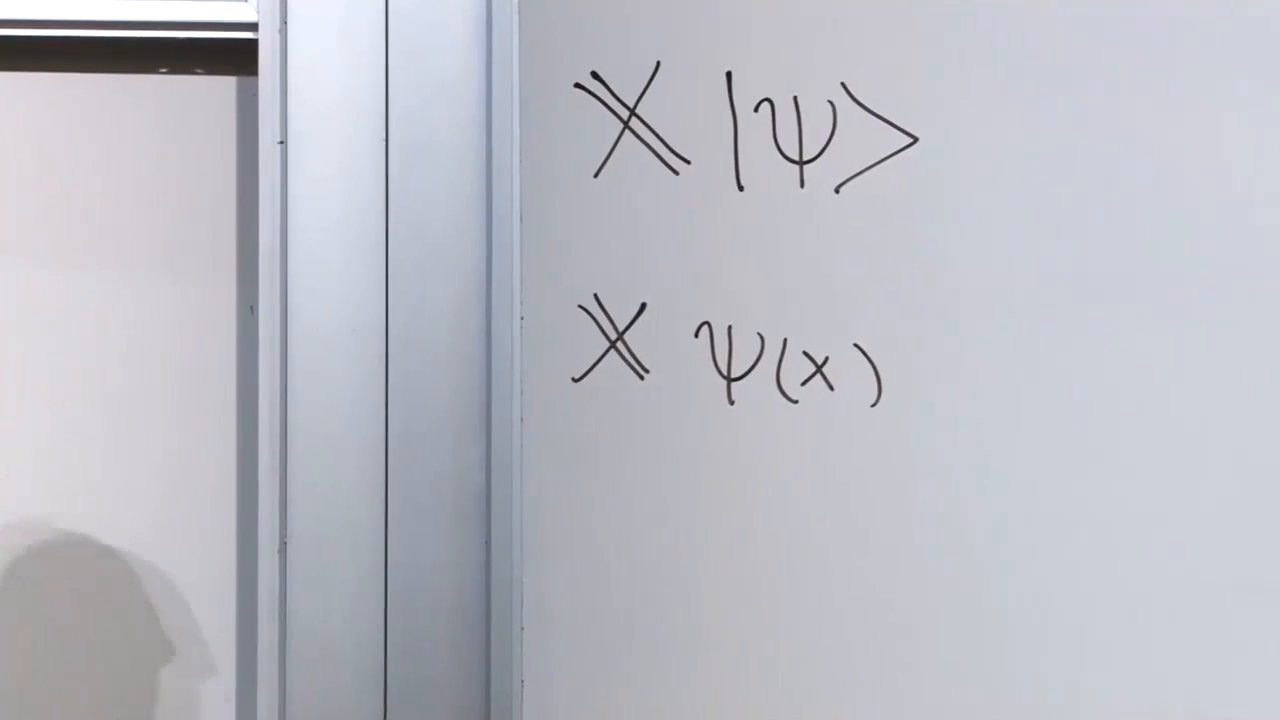
\includegraphics[width=0.88\textwidth]{lecture_09_figure_04.png}
\caption{두 변환의 합성 안에서 푸리에 핵을 분리하고, 표본 추출 작용을 이용해 이를 디랙 델타로 확인한다.}
\lectureframe{00:26:23}
\end{figure}

서로 상호적인 변수의 이름을 바꾸면 이에 대응하는 항등식을 얻는다.
\begin{equation}
\boxed{
\int_{-\infty}^{\infty}
\frac{dx}{2\pi}\,
e^{ix(p-p')}
=\delta(p-p')
}.
\label{eq:l9-delta-fourier-p}
\end{equation}
따라서 델타 함수는 평면파들의 연속 중첩이다.

\begin{classroomqa}
\audiencequestion{지수는 한 곳에서는 \(x'-x\)로, 다른 곳에서는 \(x-x'\)로 쓰였습니다. 부호가 달라지면 결과도 달라지나요?}
\lecturerresponse{아니다. 델타 함수는 짝함수다. 즉, \(\delta(u)=\delta(-u)\)이다. 따라서 차의 부호를 뒤집어도 최종 분포는 바뀌지 않는다. 중간의 지수함수는 복소켤레로 바뀌지만, 적분한 핵은 같은 델타 함수다.}
\end{classroomqa}

이 계산에는 수렴에 관한 단서가 생략되어 있다. 진동 적분은 분포이지 절대수렴하는 보통 적분이 아니며, 적분 순서를 바꾸려면 주의가 필요하다. 유한한 주기 구간을 도입하면 명료한 정칙화 방법을 얻는다. 먼저 이산 푸리에 모드와 크로네커 직교성을 사용한 다음, 구간을 무한히 늘린다. 앞의 연속 항등식은 그 극한으로 얻어진다.

\section{직선 위의 입자}

고전역학에서는 위상 공간의 한 점이 상태를 지정한다.
\begin{equation}
(x,p).
\end{equation}
양자역학은 다른 질문에서 출발한다. 상태 공간을 정의하는 정규직교 기저는 무엇인가? 각 실수 위치 \(x\)에 대해 일반화 고유켓 \(\ket{x}\)를 도입하자. 일반적인 상태는 다음과 같이 전개할 수 있다.
\begin{equation}
\ket{\Psi}
=
\int_{-\infty}^{\infty}
dx\,\psi(x)\ket{x},
\qquad
\psi(x)=\braket{x}{\Psi}.
\label{eq:l9-position-expansion}
\end{equation}

\begin{figure}[htbp]
\centering
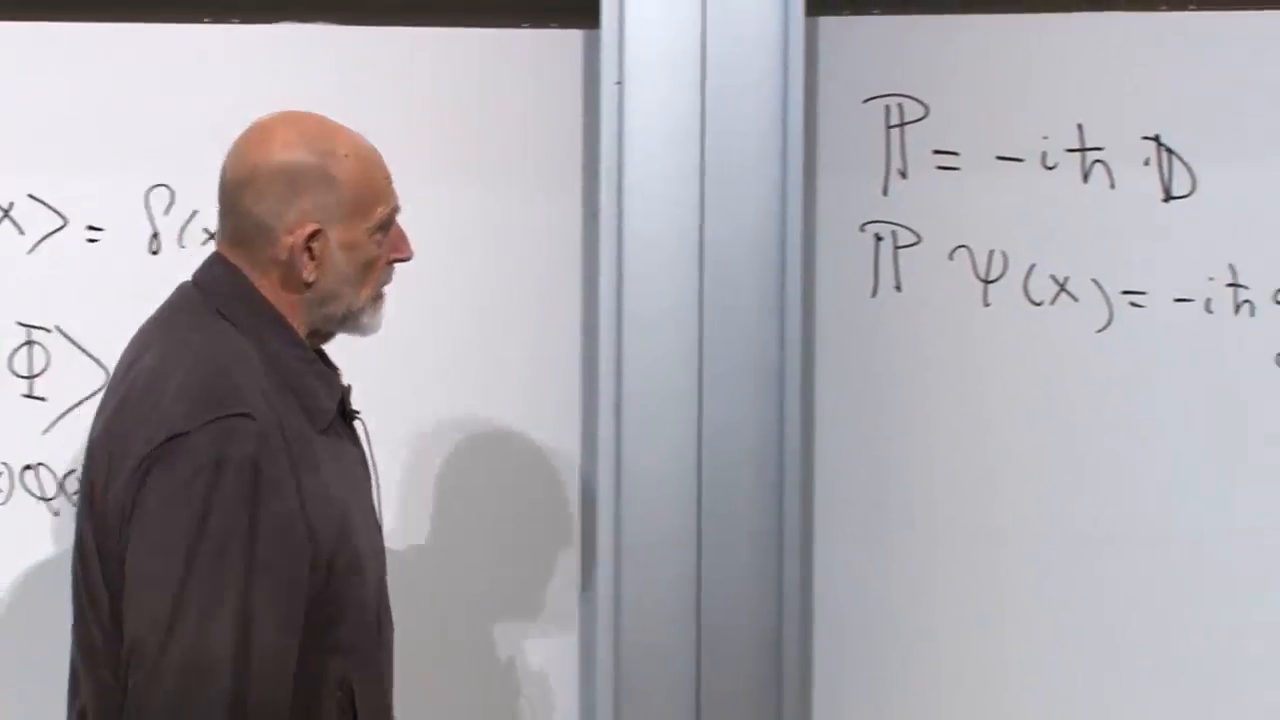
\includegraphics[width=0.88\textwidth]{lecture_09_figure_05.png}
\caption{연속 위치 기저로 전개한 일반 상태와, \(\ket{x}\)에 사영해 계수를 구하는 방법.}
\lectureframe{00:35:30}
\end{figure}

보른 규칙은 확률 밀도를 다음과 같이 정한다.
\begin{equation}
\rho(x)=|\psi(x)|^2.
\end{equation}
유한한 구간에서의 확률은 다음과 같다.
\begin{equation}
P(a<x<b)=\int_a^b|\psi(x)|^2\,dx,
\end{equation}
정규화된 물리적 상태는 다음을 만족한다.
\begin{equation}
\int_{-\infty}^{\infty}|\psi(x)|^2\,dx=1.
\label{eq:l9-position-normalization}
\end{equation}
연속 기저의 직교성은 다음과 같이 표현된다.
\begin{equation}
\braket{x'}{x}=\delta(x-x').
\label{eq:l9-position-delta}
\end{equation}
임의의 두 상태에 대한 내적은 다음과 같다.
\begin{equation}
\braket{\Psi}{\Phi}
=
\int_{-\infty}^{\infty}
dx\,\psi^*(x)\phi(x).
\label{eq:l9-position-inner-product}
\end{equation}

\begin{figure}[htbp]
\centering
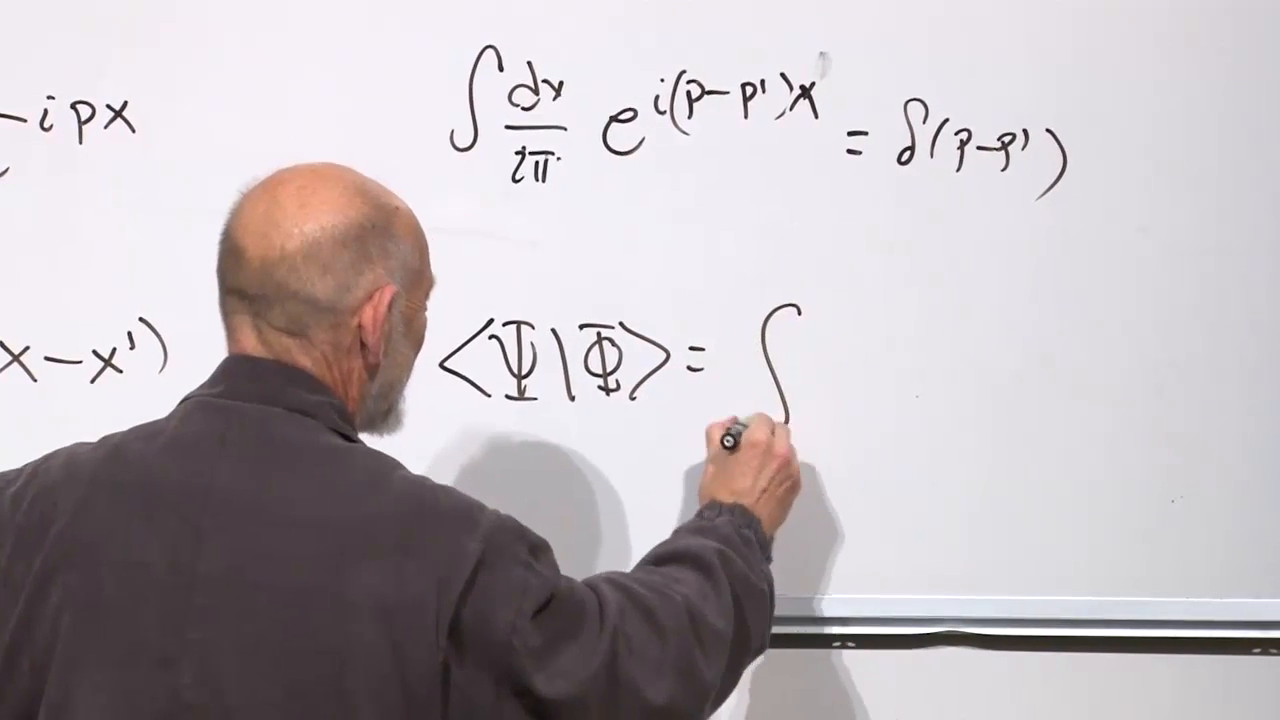
\includegraphics[width=0.88\textwidth]{lecture_09_figure_06.png}
연속 기저의 정규화와 위치 표현으로 쓴 파동 함수의 내적.\caption{
}
\lectureframe{00:41:20}
\end{figure}

\begin{classroomqa}
\audiencequestion{위치만으로 충분한 이유는 무엇인가요? 운동량이나 거의 모든 다른 변수를 더하면 중복 정보가 되나요?}
\lecturerresponse{일차원에서 입자 하나의 상태는 전체 함수 \(\psi(x)\)로 정해지므로, \(p\)의 정확한 값을 동시에 지정하면 정보가 지나치게 많아진다. 운동량은 각 \(\ket{x}\)에 덧붙이는 추가 꼬리표가 아니라 또 하나의 완전한 기저를 제공한다. 더 높은 차원에서는 서로 양립하는 정보를 함께 사용할 수 있다. 예를 들어 \(X\)와 \(P_y\)는 교환하므로 공동 기저를 표지할 수 있다. 제한의 대상은 기호의 개수 자체가 아니라 서로 교환하지 않는 쌍이다.}
\end{classroomqa}

\begin{classroomqa}
\audiencequestion{운동량도 완전한 기저를 제공하며, 위치 기저를 통해 전개할 수 있나요?}
\lecturerresponse{그렇다. 운동량 기저는 완전하며, 그 계수는 위치 계수와 푸리에 변환으로 연결된다. 이 관계가 이 강의의 핵심 구성이다.}
\end{classroomqa}

\section{위치 표현에서의 위치}

추상 연산자는 상태 벡터에 작용한다. 기저를 선택하면 같은 작용이 파동 함수에 대한 구체적인 연산으로 표현된다. 위치 표현에서 위치 연산자 \(X\)는 곱셈으로 작용한다.
\begin{equation}
(X\psi)(x)=x\psi(x).
\label{eq:l9-position-operator}
\end{equation}

\(x_0\)에 국소화된 상태는 일반화 파동 함수 \(\delta(x-x_0)\)로 표현된다. \(X\)를 적용하면 다음과 같다.
\begin{align}
X\delta(x-x_0)
&=
x\delta(x-x_0) \notag\\
&=
x_0\delta(x-x_0),
\label{eq:l9-position-eigenfunction}
\end{align}
여기서는 식~\eqref{eq:l9-delta-multiplication}을 사용했다. 따라서 \(\delta(x-x_0)\)는 고윳값 \(x_0\)을 갖는 \(X\)의 고유함수다.

\begin{figure}[htbp]
\centering
\includegraphics[width=0.88\textwidth]{lecture_09_figure_07.png}
\caption{\(x\)를 곱하면 델타 함수로 국소화된 상태는 \(x_0\)를 곱한 자기 자신이 되므로, 위치 고유함수임이 확인된다.}
\lectureframe{00:45:50}
\end{figure}

\(\ket{x_0}\)도, 이를 나타내는 델타 함수도 통상적인 제곱적분 가능성의 의미에서 노름이 1로 정규화되어 있지 않다. 이들은 델타 함수 정규화를 따른다. 물리적으로 국소화된 상태는 유한한 파동 묶음이며, 정확한 고유상태는 일반화 기저 벡터로 쓰인다.

\section{운동량 고유함수}

앞선 강의에서 미분 연산자는 반에르미트이고 \(-i\)를 곱하면 에르미트가 됨을 보았다. 단위를 복원하여 다음과 같이 정의하자.
\begin{equation}
P=-i\hbar\frac{d}{dx},
\qquad
(P\psi)(x)
=
-i\hbar\frac{d\psi}{dx}.
\label{eq:l9-momentum-operator}
\end{equation}
이는 적절한 정의역에서 정당한 관측량이다. 이를 물리적 운동량으로 식별할 수 있는지는 스펙트럼, 파장, 동역학에서의 역할을 살펴 검증할 것이다.

운동량 고윳값 \(p\)에 대해 다음을 풀자.
\begin{equation}
P\psi_p=p\psi_p,
\end{equation}
즉,
\begin{equation}
-i\hbar\frac{d\psi_p}{dx}=p\psi_p.
\end{equation}
해는 다음과 같다.
\begin{equation}
\psi_p(x)=A e^{ipx/\hbar}.
\label{eq:l9-momentum-eigenfunction}
\end{equation}

\begin{figure}[htbp]
\centering
\includegraphics[width=0.88\textwidth]{lecture_09_figure_08.png}
\caption{운동량이 정해진 상태를 위치 공간에서 나타내면 평면파 \(e^{ipx/\hbar}\)가 된다.}
\lectureframe{00:51:45}
\end{figure}

파장 \(\lambda\)는 위상이 \(2\pi\)만큼 증가하는 변위다.
\begin{equation}
\frac{p\lambda}{\hbar}=2\pi,
\qquad
\lambda=\frac{2\pi\hbar}{p}.
\label{eq:l9-de-broglie}
\end{equation}
따라서 운동량이 클수록 파장은 짧다.

델타 함수 정규화로 상수를 정할 수 있다.
\begin{equation}
\psi_p(x)
=
\frac{1}{\sqrt{2\pi\hbar}}e^{ipx/\hbar}.
\label{eq:l9-normalized-momentum-eigenfunction}
\end{equation}
실제로,
\begin{align}
\braket{p'}{p}
&=
\int_{-\infty}^{\infty}
dx\,
\psi_{p'}^*(x)\psi_p(x) \notag\\
&=
\int_{-\infty}^{\infty}
\frac{dx}{2\pi\hbar}
e^{i(p-p')x/\hbar} \notag\\
&=
\delta(p-p').
\label{eq:l9-momentum-normalization}
\end{align}
\(\hbar=1\)로 두는 단위계를 택하면 이 식들은 다음과 같이 된다.
\begin{equation}
\psi_p(x)=\frac{1}{\sqrt{2\pi}}e^{ipx},
\qquad
\int\frac{dx}{2\pi}e^{i(p-p')x}
=\delta(p-p').
\end{equation}

\begin{classroomqa}
\audiencequestion{보통의 의미로는 수렴하지 않는데, \(p\neq p'\)일 때 진동 적분을 어떻게 0이라고 할 수 있나요?}
\lecturerresponse{강의에서는 계산을 통제된 방식으로 간략화한다. 계를 유한한 주기 구간에 둔다. 그러면 허용되는 운동량은 이산적인 집합을 이루고 지수함수들은 통상적인 의미에서 직교하며, 모든 정규화가 유한하다. 그 계산을 마친 뒤에야 구간을 무한대로 보내 크로네커 델타를 디랙 델타로 바꾼다.}
\end{classroomqa}

\begin{classroomqa}
\audiencequestion{델타 함수의 푸리에 변환 유도에도 같은 수렴 문제가 있나요?}
\lecturerresponse{그렇다. 같은 이유로 그곳에서 적분 순서를 바꾼 것은 형식적인 계산이었다. 유한 상자를 이용한 유도나 분포의 언어가 생략된 엄밀성을 보완한다. 정칙화한 계산이 언급된 연속 극한을 갖기 때문에 이 간략화는 허용된다.}
\end{classroomqa}

\section{운동량 표현}

두 대상을 혼동해서는 안 된다. 식~\eqref{eq:l9-normalized-momentum-eigenfunction}의 함수 \(\psi_p(x)\)는 특정 고유상태 \(\ket{p}\)를 위치 공간에서 나타낸 것이다. 반면 임의의 상태 \(\ket{\Psi}\)의 운동량 공간 파동 함수는 다음과 같다.
\begin{equation}
\widetilde{\psi}(p)=\braket{p}{\Psi}.
\label{eq:l9-momentum-wavefunction}
\end{equation}
\(\bra{p}\)와 \(\ket{\Psi}\)의 위치 공간 파동 함수를 대입하자.
\begin{align}
\widetilde{\psi}(p)
&=
\int_{-\infty}^{\infty}
dx\,
\braket{p}{x}\braket{x}{\Psi} \notag\\
&=
\int_{-\infty}^{\infty}
\frac{dx}{\sqrt{2\pi\hbar}}\,
e^{-ipx/\hbar}\psi(x).
\label{eq:l9-position-to-momentum}
\end{align}
이것이 바로 푸리에 변환이다. 반대로,
\begin{equation}
\psi(x)
=
\int_{-\infty}^{\infty}
\frac{dp}{\sqrt{2\pi\hbar}}\,
\widetilde{\psi}(p)e^{ipx/\hbar}.
\label{eq:l9-momentum-to-position}
\end{equation}

\begin{figure}[htbp]
\centering
\includegraphics[width=0.88\textwidth]{lecture_09_figure_09.png}
\caption{\(\ket{p}\)에 사영하면 위치 공간 파동함수는 푸리에 변환 \(\widetilde{\psi}(p)\)으로 바뀐다.}
\lectureframe{01:05:50}
\end{figure}

운동량 \(p\)을 측정할 확률 밀도는 다음과 같다.
\begin{equation}
\widetilde{\rho}(p)
=
|\widetilde{\psi}(p)|^2,
\qquad
\int_{-\infty}^{\infty}
|\widetilde{\psi}(p)|^2\,dp=1.
\end{equation}
따라서 위치 공간 파동 함수 하나에 위치와 운동량 측정을 모두 예측하는 데 필요한 정보가 충분히 담겨 있다. 운동량 확률을 구하려면 \(\psi(x)\)를 푸리에 변환한 다음 그 결과의 절댓값을 제곱하면 된다.

운동량 표현에서는 역할이 서로 바뀐다.
\begin{equation}
(P\widetilde{\psi})(p)
=
p\widetilde{\psi}(p),
\qquad
(X\widetilde{\psi})(p)
=
i\hbar\frac{d\widetilde{\psi}}{dp}.
\label{eq:l9-operators-in-p}
\end{equation}
\(P=-i\hbar\,d/dx\)와 부호가 다른 것은 푸리에 쌍에서 지수의 부호가 서로 반대이기 때문이다.

\begin{classroomqa}
\audiencequestion{시간은 위치와 운동량의 관계처럼 에너지에 켤레인 연산자인가요?}
\lecturerresponse{시간은 보통 계의 상태 진화를 나타내는 외부 매개변수로 다루며, 계의 힐베르트 공간에서 보편적인 자기수반 연산자로 다루지는 않는다. 물리적 시계에는 관측 가능한 눈금이 있고, 시계의 시간 분해능을 높이면 에너지에 영향을 주지만, 시간-에너지 관계는 위치-운동량 쌍보다 더 신중히 다뤄야 하므로 여기서는 전개하지 않는다.}
\end{classroomqa}

\begin{classroomqa}
\audiencequestion{그 밖에 어떤 켤레 쌍이 있나요?}
\lecturerresponse{각도와 이에 대응하는 각운동량이 중요한 예이며, 각도가 주기 변수라는 점에서 전역적인 단서가 따른다. 장론에서는 장과 그 정준 운동량이 켤레 관계다. 온도와 압력은 열역학 변수이지 정준 양자 쌍이 아니다. 일반 원리는 임의의 두 측정 가능량에서 나오는 것이 아니라 정준 변수와 그 교환자에서 나온다.}
\end{classroomqa}

\begin{classroomqa}
\audiencequestion{이산 이론에서는 연산자가 켓에 작용하고 파동 함수는 계수만 나열했습니다. 연속 이론에서는 달라졌나요?}
\lecturerresponse{아니다. 파동 함수는 선택한 기저에서 추상적 켓을 나타내는 좌표 열벡터다. 유한한 열벡터에 작용하는 행렬과 함수에 작용하는 미분 또는 적분 연산자는 같은 추상적 작용을 구체적으로 표현한 것이다. 연속 변수는 표기를 바꿀 뿐 논리는 바꾸지 않는다.}
\end{classroomqa}

\subsection{푸리에 변환에서 비롯되는 불확정성}

운동량이 정해진 상태는 공간 전체에 완전히 퍼져 있다.
\begin{equation}
|\psi_p(x)|^2=\text{constant}.
\end{equation}
운동량은 정확히 정해져 있지만, 위치는 직선 전체에 균일하게 퍼져 있다. 더 일반적으로 푸리에 쌍인 두 함수는 동시에 좁은 범위에 모일 수 없다. \(\widetilde{\psi}(p)\)를 좁은 운동량 범위에 집중시키면 \(\psi(x)\)는 넓은 영역으로 퍼져야 하고, \(\psi(x)\)를 국소화하려면 넓은 운동량 범위가 필요하다.

강의에서는 아직 정량적 부등식을 유도하지 않는다.
\begin{equation}
\Delta X\,\Delta P\geq\frac{\hbar}{2}.
\end{equation}
여기서 강조하는 점은 구조적이다. 불확정성 원리는 푸리에 변환의 상호적 기하에 이미 담겨 있다. 이는 양립할 수 없는 스핀 기저 사이의 변환에 대응하는 연속적인 경우다.

\section{시간 진화를 생성하는 해밀토니안}

해밀토니안 \(H\)은 에르미트 연산자이며 에너지를 나타내고 유니터리 시간 진화를 생성한다. 시간 의존 Schr\"odinger 방정식은 다음과 같다.
\begin{equation}
i\hbar\frac{d}{dt}\ket{\Psi(t)}
=
H\ket{\Psi(t)}.
\label{eq:l9-abstract-schrodinger}
\end{equation}
위치 표현에서는 다음과 같다.
\begin{equation}
i\hbar\frac{\partial\psi(x,t)}{\partial t}
=
H\psi(x,t),
\label{eq:l9-position-schrodinger}
\end{equation}
여기서 우변은 해밀토니안이 함수에 작용한 결과를 위치 공간에서 표현한 것이다.

\subsection{의도적으로 단순화한 선형 해밀토니안}

다음과 같이 두자.
\begin{equation}
H=cP.
\label{eq:l9-linear-hamiltonian}
\end{equation}
이는 통상적인 비상대론적 자유입자 해밀토니안이 아니다. 모든 단계를 직접 확인할 수 있도록 택한 것이다.

\begin{figure}[htbp]
\centering
\includegraphics[width=0.88\textwidth]{lecture_09_figure_10.png}
\caption{Schr\"odinger 방정식과 선형 해밀토니안 \(H=cP\): 입자의 시간 발전을 설명하는 가장 단순한 예로 선택했다.}
\lectureframe{01:17:45}
\end{figure}

\(P=-i\hbar\,\partial_x\)를 사용하면,
\begin{align}
i\hbar\frac{\partial\psi}{\partial t}
&=
c\left(-i\hbar\frac{\partial}{\partial x}\right)\psi, \notag\\
\frac{\partial\psi}{\partial t}
&=
-c\frac{\partial\psi}{\partial x},
\end{align}
즉,
\begin{equation}
\frac{\partial\psi}{\partial t}
+c\frac{\partial\psi}{\partial x}=0.
\label{eq:l9-transport-equation}
\end{equation}

\begin{figure}[htbp]
\centering
\includegraphics[width=0.88\textwidth]{lecture_09_figure_11.png}
\caption{선형 해밀토니안은 Schr\"odinger 방정식을 일차 수송 방정식으로 바꾼다.}
\lectureframe{01:20:05}
\end{figure}

일반해는 다음과 같다.
\begin{equation}
\psi(x,t)=f(x-ct),
\label{eq:l9-rigid-translation}
\end{equation}
여기서 \(f\)는 정규화 가능한 임의의 초기 분포다. \(t=0\)에서 분포는 \(f(x)\)다. 이후에는 모든 특징이 오른쪽으로 \(ct\)만큼 이동한다. 복소 파동 함수와 그 실수부 및 허수부, 확률 밀도는 모두 형태를 유지한다.
\begin{equation}
|\psi(x,t)|^2=|f(x-ct)|^2.
\end{equation}
따라서 다음이 성립한다.
\begin{equation}
\expect{X}_t=\expect{X}_0+ct.
\end{equation}

기호 \(c\)는 빛의 속도를 연상하도록 택했다. 이 모형은 한 방향으로 한 속도로 움직이는 1차원 카이랄 질량 없는 들뜸 하나와 비슷하다. 완전한 광자 이론은 아니다. 고정된 음속을 갖는 저에너지 1차원 포논도 비슷한 사례다. \(E=cp\)이므로 \(p\)의 양쪽 부호를 모두 허용하면 음의 에너지도 생긴다. 이 역시 의도적으로 범위를 제한한 교육용 모형임을 보여 준다.

\begin{classroomqa}
\audiencequestion{\(H=cP\)에서 \(c\)를 그 입자의 속도로 바꾸면 자유 입자를 나타낼 수 있나요?}
\lecturerresponse{아니요. \(H=cP\)에서 계수는 고정되어 있으므로 모든 운동량 성분이 같은 속도를 갖는다는 뜻입니다. 비상대론적 입자의 속도는 \(p/m\)이므로 운동량에 따라 달라집니다. \(vP\)에 \(v=p/m\)을 대입하면 더 이상 \(P\)에 대해 선형이 아니며, 이는 이차 해밀토니안으로 이어집니다.}
\end{classroomqa}

\begin{classroomqa}
\audiencequestion{보통 자유롭게 움직이는 전자의 파동 함수도 단지 형태를 유지한 채 이동해야 하지 않나요?}
\lecturerresponse{모든 분포를 형태 그대로 이동시키는 것은 매우 특수한 분산 관계에서만 가능하다. 보통의 자유전자 파동 묶음은 위상이 서로 다른 비율로 변하는 여러 운동량 성분을 포함한다. 중심은 이동하지만, 일반적으로 형태는 퍼진다.}
\end{classroomqa}

\subsection{고전역학과의 비교}

고전 해밀토니안 \(H=cp\)에 대해 해밀턴 방정식은 다음과 같다.
\begin{equation}
\dot{x}=\frac{\partial H}{\partial p}=c,
\qquad
\dot{p}=-\frac{\partial H}{\partial x}=0.
\label{eq:l9-linear-hamilton-equations}
\end{equation}

\begin{figure}[htbp]
\centering
\includegraphics[width=0.88\textwidth]{lecture_09_figure_12.png}
\caption{\(H=cp\)에 대한 해밀턴 방정식: 오른쪽으로 일정한 속도로 움직이며 운동량은 보존된다.}
\lectureframe{01:25:20}
\end{figure}

양자 확률 분포와 그 기댓값은 같은 기본적인 운동을 따른다. 이는 고전 해밀토니안으로 구성한 양자 시간 진화가 적절한 의미에서 고전 방정식을 재현해야 한다는 점을 구체적으로 보여 주는 첫 사례다.

\section{비상대론적 자유입자}

힘을 받지 않는 질량 \(m\)의 보통 입자에 대해 고전적인 운동에너지는 다음과 같다.
\begin{equation}
H=\frac{p^2}{2m}.
\end{equation}
이 이차식에서는 \(p\)와 \(-p\)가 대칭적으로 취급되므로, 왼쪽으로 움직이는 입자와 오른쪽으로 움직이는 입자는 같은 양의 에너지를 갖는다. 양자화할 때 \(p\)를 연산자 \(P\)로 바꾼다.
\begin{equation}
H=\frac{P^2}{2m}.
\label{eq:l9-free-hamiltonian}
\end{equation}
\(P=-i\hbar\,\partial_x\)를 Schr\"odinger 방정식에 대입하면 다음과 같다.
\begin{align}
i\hbar\frac{\partial\psi}{\partial t}
&=
\frac{1}{2m}
\left(-i\hbar\frac{\partial}{\partial x}\right)^2
\psi \notag\\
&=
-\frac{\hbar^2}{2m}
\frac{\partial^2\psi}{\partial x^2}.
\label{eq:l9-free-schrodinger}
\end{align}

\begin{figure}[htbp]
\centering
\includegraphics[width=0.88\textwidth]{lecture_09_figure_13.png}
\caption{Schr\"odinger 방정식은 \(H=P^2/(2m)\)과 \(P=-i\hbar\,\partial_x\)에서 얻는다.}
\lectureframe{01:33:50}
\end{figure}

운동량이 \(p\)인 평면파 성분의 에너지는 다음과 같다.
\begin{equation}
E(p)=\frac{p^2}{2m}.
\end{equation}
선형인 경우 \(E=cp\)와 달리, 이 분산 관계의 기울기는 \(p\)에 따라 달라진다.
\begin{equation}
v_{\mathrm{group}}
=
\frac{dE}{dp}
=
\frac{p}{m}.
\end{equation}
따라서 국소화된 파동 묶음의 운동량 성분들은 서로 다른 군속도로 움직인다. 성분들 사이의 상대 위상이 변하고, 성분들은 서로 멀어지면서 파동 묶음이 퍼진다. 핵심적인 차이는 \(H=cP\)가 모든 형태를 그대로 이동시키는 반면, \(H=P^2/(2m)\)은 분산을 동반한 자유입자 운동을 일으킨다는 것이다.

\section{확립한 내용}

수학적 논의는 물리학과 별개가 아니었다. 평면파와 디랙 델타를 통해 연속 기저를 구성하는 도구를 마련했다. 위치 연산자는 곱셈으로, 운동량 연산자는 미분으로 작용하며, 운동량 고유상태는 평면파다. 임의의 상태를 이 고유상태들에 사영하면 위치 파동 함수의 푸리에 변환을 얻는다. 따라서 위치와 운동량은 하나의 상태를 나타내는 서로 다른 두 표현이며, 불확정성은 푸리에 쌍의 폭이 서로 반비례한다는 익숙한 사실이다.

같은 표현 도구를 사용하면 해밀토니안은 미분 방정식으로 바뀐다. 운동량의 선형 함수는 형태를 유지하는 평행이동을 만들고, 이차 운동에너지는 자유입자의 Schr\"odinger 방정식과 분산을 만든다. 강의는 측정의 기초에서 운동의 역학으로 나아갔지만, 상태, 기저, 에르미트 관측량, 진폭, 유니터리 시간 진화라는 중심 언어는 그대로 유지했다.
